\section{Determinante einer Matrix}

\begin{remark}
	Wir werden nun auch Matrizen mit Koeffizienten in Ring $R$ anstatt $K$ betrachten. Mit der gewohnten Addition und 
	Multiplikation bilden die $n\times n$-Matrizen einen Ring $\Mat_n(R)$, und wir definieren wieder $\GL_n(R)=\Mat_n(R)^{\times}$.
\end{remark}

\begin{remark}
	Seien $a_1,...,a_n\in R^m$ Spaltenvektoren, so bezeichnen wir mit $A=(a_1,...,a_n)\in \Mat_{m\times n}(R)$ die 
	Matrix mit den Spalten $a_1,...,a_n$. sind $\widetilde{a_1},...,\widetilde{a_m}\in R^n$ Zeilenvektoren, so bezeichnen wir mit $\tilde A=(
	\widetilde{a_1},...,\widetilde{a_m})\in \Mat_{m\times n}(R)$ die Matrix mit den Zeilen $\widetilde{a_1},...,\widetilde{a_m}$.
\end{remark}

\begin{remark}
	\proplbl{4_2_3}
	Wir hatten bereits definiert: $\det(A)=ad-bc$ (\propref{3_1_13}) mit 
	\begin{align}
		A=\begin{pmatrix}a&b\\c&d\end{pmatrix}\in \Mat_2(K)\notag
	\end{align} und hatten 
	festgestellt: $\det(A)\neq 0 \iff A\in \GL_2(K)$. Interpretation im $K=\mathbb R$:\\
	\begin{center}
		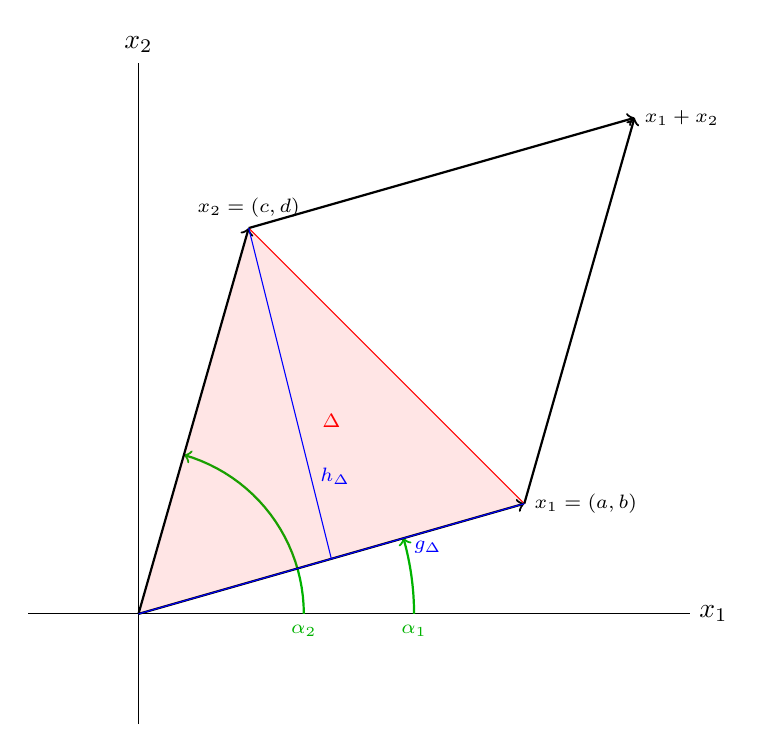
\begin{tikzpicture}[scale=0.7]
		\draw[thin] (-2,0) -- (10,0) node[right] {$x_1$}; 
		\draw[thin] (0,-2) -- (0,10) node[above] {$x_2$};
		%circles
		\draw [->,green!70!black,thick,domain=0:16] plot ({5*cos(\x)}, {5*sin(\x)});
		\draw [green!70!black] (5,-0.3) node {\scriptsize $\alpha_1$};
		\draw [->,green!70!black,thick,domain=0:74] plot ({3*cos(\x)}, {3*sin(\x)});
		\draw [green!70!black] (3,-0.3) node {\scriptsize $\alpha_2$};
		% triangle
		\fill[line width=1pt, color=red,fill=red, opacity=0.1] (0,0) -- (2,7) -- (7,2) -- cycle ;
		\draw[red] (2,7) -- (7,2);
		\draw[red] (3.5,3.5) node {\scriptsize $\Delta$};
		% Paralello
		\draw[->, thick] (0,0) -- (7,2) node[right] {\scriptsize $x_1=(a,b)$};
		\draw[->, thick] (0,0) -- (2,7) node[above] {\scriptsize$x_2=(c,d)$};
		\draw[->, thick] (7,2) -- (9,9) node[right] {\scriptsize$x_1 + x_2$};
		\draw[->, thick] (2,7) -- (9,9);
		\draw[blue] (0,0) -- (7,2) node[near end, below] {\scriptsize $g_{\Delta}$};
		\draw[blue] (3.5,1) -- (2,7) node[near start, right] {\scriptsize$h_{\Delta}$};
		\end{tikzpicture}
	\end{center}
	Parallelogramm hat die Fläche $|\det A|$. Polarkoordinaten: $x_i=\lambda_i(\cos a_i, \sin a_i)$. Ohne Einschränkung: $0\le a_1 \le a_2
	\le \pi$
	\begin{align}
	F_{P} &= 2\cdot F_{\Delta} = 2\cdot \frac 1 2 \cdot g_{\Delta} \cdot h_{\Delta} \notag \\
	g_{\Delta} &= \lambda_1 \notag \\
	h_{\Delta} &= \lambda_2 \cdot \sin(a_2-a_1) \notag \\
	F_{P} &= \lambda_1\lambda_2(\cos a_1 \sin a_2 - \sin a_1 \cos a_2) = \det(\begin{pmatrix}\lambda_1 \cos a_1 & 
	\lambda_1 \sin a_1 \\ \lambda_2 \cos a_2 & \lambda_2 \sin a_2 \end{pmatrix}) \notag \\
	&= \det A \notag
	\end{align}
	Insbesondere erfüllt $\det$ die folgenden Eigenschaften: 
	\begin{itemize}
		\item Für $\lambda\in R$ ist $\det(\lambda x_1,x_2)=\det(x_1,\lambda x_2)=\lambda\cdot \det(x_1,x_2)$
		\item Für $x_i=x'_i+x''_i$ ist $\det(x_1,x_2)=\det(x'_1,x_2) + \det(x''_1,x_2)$
		\item Ist $x_1=x_2$, so ist $\det A=0$
		\item $\det(\mathbbm{1}_2)=1$
	\end{itemize}
\end{remark}

\begin{definition}[Determinantenabbildung]
	Eine Abbildung $\delta:\Mat_n(R)\to R$ heißt \begriff{Determinantenabbildung}, wenn gilt:
	\begin{itemize}
		\item (D1): $\delta$ ist linear in jeder Zeile: sind $a_1,...,a_n$ die Zeilen von $A$ und ist $i\in \{1,...,n\}$ und $a_i=\lambda'a'_i + 
		\lambda''a''_i$ mit $\lambda',\lambda''\in R$ und den Zeilenvektoren $a'_i,a''_i$, so ist $\delta(A)=\lambda'\cdot \delta(a_1,...,
		a'_i,...,a_n) + \lambda''\cdot \det(a_1,...,a''_i,...,a_n)$.
		\item (D2): $\delta$ ist alternierend: sind $a_1,...,a_n$ die Zeilen von $A$ und $i,j\in \{1,...,n\}$, $i\neq j$ mit $a_i=a_j$, so ist 
		$\delta(A)=0$.
		\item (D3): $\delta$ ist normiert: $\delta(\mathbbm{1}_n)=1$.
	\end{itemize}
\end{definition}

\begin{mathematica}[Determinante]
	Die Determinante einer Matrix lässt sich in Mathematica bzw. WolframAlpha wie folgt berechnen:
	\begin{align}
		\texttt{Det[\{\{1, 4\}, \{2, 5\}\}]}\notag
	\end{align}
\end{mathematica}

\begin{example}
	\proplbl{4_2_5}
	Sei $\delta:\Mat_n(K)\to K$ eine Determinantenabbildung. Ist $A\in \Mat_n(K)$ nicht invertierbar, so sind die Zeilen 
	$a_1,...,a_n$ von $A$ linear abhängig, es gibt also ein $i$ mit $a_i=\sum_{j\neq i} \lambda_j\cdot a_j$. Es folgt $\delta(A)=
	\delta(a_1,...,a_n)=\sum_{j\neq i} \lambda_j\cdot \delta(a_1,...,a_j,...,a_n)$ mit $a_i=a_j$ mit D2: $\sum_{j\neq i} 
	\lambda_j\cdot 0=0=\delta(A)$.
\end{example}

\begin{lemma}
	\proplbl{4_2_6}
	Erfüllt $\delta:\Mat_n(R) \to R$ die Axiome D1 und D2, so gilt für jedes $\sigma\in S_n$ und die Zeilenvektoren 
	$a_1,...,a_n$: 
	\begin{align}
		\delta(a_{\sigma(1)},...,a_{\sigma(n)})=\sgn(\sigma)\cdot \delta(a_1,...,a_n)\notag
	\end{align}
\end{lemma}
\begin{proof}
	 $\sigma$ ist ein Produkt von Transpositionen. Es genügt also die Behauptung für $\sigma=\tau_{ij}$ mit $1\le i<j\le n$ zu zeigen (\propref{4_1_7}). \\
	 \begin{align}
	 	0&=\delta(a_1,...,a_i+a_j,...,a_j+a_i,....,a_n) \notag \\
	 	&=\delta(a_1,...,a_i,...,a_j,...,a_n)+\delta(a_1,...,a_i,...,a_i,...,a_n)+\delta(a_1,...,a_j,
	 	...,a_j,...,a_n)+\delta{a_1,...,a_j,...,a_i,...,a_n} \notag \\
	 	&=\delta(a_1,...,a_n)+\delta(a_{\sigma(1)},...,a_{\sigma(n)}) \notag \\
	 	&=0 \notag
	 \end{align}
	 Mit $\sgn(\sigma)=
	 \sgn(\tau_{ij})=-1$ folgt die Behauptung.
\end{proof}

\begin{lemma}
	\proplbl{4_2_7}
	Erfüllt $\delta:\Mat_n(R)\to R$ die Axiome D1 und D2, so gilt für $A=(a_{ij})\in \Mat_n(R)$: 
	\begin{align}
		\delta(A)=\delta(\mathbbm{1}_n)
		\cdot \sum_{\sigma\in S_n} \left( \prod_{i=1}^n a_{i,\sigma(i)} \right)\notag
	\end{align}
\end{lemma}
\begin{proof}
	Schreibe $a_i=(a_{j_1},...,a_{in})=\sum_{j=1}^n a_{ij}\cdot e_j$. Wiederholtes Anwenden von D1 gibt 
	\begin{align}
		\delta(A)&=\delta(a_1,...,a_n) \notag \\
		&=\sum_{j_1=1}^n a_{1j_1}\cdot \delta(e_{j_1},a_2,...,a_n) \notag \\
		&=\sum_{j_1=1}^n ... \sum_{j_n=1}^n \delta(e_{j_1},...,e_{j_n})\cdot \prod_{i=1}^n a_{ij_i} \notag
	\end{align}
	Wegen D2 ist $\delta(e_{j_1},...,e_{j_n})=0$ falls $j_i=j_{i'}$ für ein $i\neq i'$. 
	Andernfalls ist $\sigma(i)=j_i$ einer Permutation von $\{1,...,n\}$ und 
	\begin{align}
		\delta(e_{j_1},...,e_{j_n})&=\delta(e_{\sigma(1)},...,e_{\sigma(n)}) \notag \\
		&=\sgn(\sigma)\cdot \delta(e_1,...,e_n) \notag \\
		&=\sgn(\sigma)\cdot \delta(\mathbbm{1}_n) \notag
	\end{align}
	nach \propref{4_2_6}.
\end{proof}

\begin{theorem}
	\proplbl{4_2_8}
	Es gibt genau eine Determinantenabbildung $\delta:\Mat_n(R)\to R$ und diese ist gegeben durch die 
	Leibnitzformel 
	\begin{align}
		\det(a_{ij})=\sum_{\sigma\in S_n} \sgn(\sigma)\cdot \prod_{i=1}^n a_{i,\sigma(i)} = \sum_{\sigma
			\in A_n}\prod_{i=1}^n a_{i,\sigma(i)} - \sum_{\sigma\in S_n\backslash A_n}\prod_{i=1}^n a_{i,\sigma(i)}\notag
	\end{align}
\end{theorem}
\begin{proof}
	Eindeutigkeit der Abbildung folgt wegen D3 aus \propref{4_2_7}. Bleibt nur noch zu zeigen, dass $\det$ auch die Axiome D1 bis D3 erfüllt. \\
	D1: klar \\
	D3: klar \\
	D2: Seien $\mu\neq v$ mit $a_{\mu}=a_v$. Mit $\tau=\tau_{\mu v}$ ist $S_n\backslash A_n = A_n\tau$, somit 
	\begin{align}
		\det(a_{ij})&=
		\sum_{\sigma\in A_n} \prod_{i=1}^n a_{i,\sigma(i)}-\sum_{\sigma\in A_n\tau} \prod_{i=1}^n a_{i,\sigma\tau(i)} \notag \\
		&=
		\sum_{\sigma\in A_n} \left( \prod_{i=1}^n a_{i,\sigma(i)} - \prod_{i=1}^n a_{i,\sigma\tau(i)} \right) \notag
	\end{align}
	nach \propref{4_1_10}. Da $a_{ij}=a_{\tau(i),j}$ 
	für alle $i,j$ ist 
	\begin{align}
		\prod_{i=1}^n a_{i,\sigma(i)}&=\prod_{i=1}^n a_{\tau(i),\sigma\tau(i)} \notag \\
		&=\prod_{i=1}^n a_{i,\sigma\tau(i)} \notag
	\end{align}
	für jedes $\sigma\in S_n$, woraus $\det(a_{ij})=0$ folgt.
\end{proof}

\begin{example}
	\proplbl{4_2_9}
	\begin{itemize}
		\item $n=2$, $S_2=\{\id, \tau_{12}\}$, 
		\begin{align}
			A=\begin{pmatrix}a_{11} & a_{12} \\ a_{21}  & a_{22}\end{pmatrix}\notag
		\end{align}
		$\det(A)=\sum_{\sigma\in
			S_2} a_{1,\sigma(1)}\cdot a_{2,\sigma(2)}=a_{11}\cdot a_{22} - a_{12}\cdot a_{21}$
		\item $n=3$, $S_3=\{id,\tau_{12}, \tau_{23}, \tau_{13}, \text{2 zyklische Vertauschungen}\}$, $A_3=\{\id, \text{2 zyklische 
			Vertauschungen}\}$, $S_3\backslash A_3=\{\tau_{12},\tau_{23},\tau_{13}\}$ und
		\begin{align}
			A=\begin{pmatrix}
			a_{11} & a_{12} & a_{13} \\
			a_{21} & a_{22} & a_{23} \\
			a_{31} & a_{32} & a_{33} \\
			\end{pmatrix}\notag
		\end{align}
		ergibt sich: $\det(A)=\sum_{\sigma\in A_3} a_{1,\sigma(1)}\cdot a_{2,\sigma(2)}\cdot a_{3,\sigma(3)} - \sum_
		{\sigma\in S_3\backslash A_3} a_{1,\sigma(1)}\cdot a_{2,\sigma(2)}\cdot a_{3,\sigma(3)}= a_{11}a_{22}a_{33} + a_{12}a_{23}
		a_{31} + a_{13}a_{21}a_{32} - a_{12}a_{21}a_{33} - a_{13}a_{22}a_{31} - a_{11}a_{23}a_{32}$
		\item Ist $A=(a_{ij})$ eine obere Dreiecksmatrix, so ist $\det(A)=\prod_{i=1}^n a_{ii}$
		\item Für $i\neq j$, $\lambda\in K^{\times}$, $\mu\in K$ ist $\det(S_i(\lambda))=\lambda$, $\det(Q_{ij}(\mu))=1$, $\det(P_{ij})=-1$
		\item Ist $A$ eine \begriff{Blockmatrix} der Gestalt 
		\begin{align}
			\begin{pmatrix}A_1 & C \\ 0 & A_2\end{pmatrix}\notag
		\end{align} mit quadratischen Matrizen $A_1,
		A_2,C$, so ist $\det(A)=\det(A_1)\cdot \det(A_2)$
	\end{itemize}
\end{example}

\begin{conclusion}
	Für $A\in \Mat_n(R)$ ist $\det(A)=\det(A^t)$. Insbesondere erfüllt $\det$ die Axiome D1 und D2 auch für Spalten 
	anstatt Zeilen.
\end{conclusion}
\begin{proof}
	Mit $\rho=\sigma^{-1}$ gilt $\sgn(\rho)=\sgn(\sigma)$ nach \propref{4_1_8} und somit 
	\begin{align}
		\det(A)&=\sum_{\sigma\in S_n} \sgn(\sigma) \cdot \prod_
		{i=1}^n a_{i,\sigma(i)} \notag \\
		&=\sum_{\rho\in S_n} \sgn(\rho)\cdot \prod_{i=1}^n a_{\rho(i),i} \notag \\
		&=\det(A^t) \notag
	\end{align}
	nach \propref{4_2_8}.
\end{proof}

\begin{theorem}[Determinantenmultiplikationssatz]
	\proplbl{4_2_11}
	Für $A,B\in \Mat_n(R)$ ist 
	\begin{align}
		\det(AB)=\det(A)\cdot \det(B)\notag
	\end{align}
\end{theorem}
\begin{proof}
	Fixiere $A$ und betrachte die Abbildung $\delta: \Mat_n(R)\to R$ mit $B\mapsto \det(AB^{-1})$. Diese Abbildung erfüllt die Axiome 
	D1 und D2. sind $b_1,...,b_n$ die Zeilen von $B$, so hat $AB^{-1}$ die Spalten $Ab_1^t,...,Ab_n^t$, es werden die Eigenschaften 
	von $\det$ auf $\delta$ übertragen. \\
	$\Rightarrow \det(AB)=\delta(B^t)=\delta(\mathbbm{1}_n)\cdot \det(B^t)=\det(A)\cdot \det(B)$.
\end{proof}

\begin{conclusion}
	\proplbl{4_2_12}
	Die Abbildung $\det:\Mat_n(R)\to R$ schränkt sich zu einem Gruppenhomomorphismus $\GL_n(R)\to 
	R^{\times}$ ein. Ist $R=K$ ein Körper, so ist $A\in \Mat_n(K)$ also genau dann invertierbar, wenn $\det(A)\neq 0$ und in 
	diesem Fall ist $\det(A^{-1})=\det(A)^{-1}$.
\end{conclusion}
\begin{proof}
	Aus $AA^{-1}=\mathbbm{1}_n$ folgt $\det(A^{-1})*\det(A)=\det(\mathbbm{1}_n)=1$, insbesondere $\det(A)\in R^{\times}$. Der zweite Teil folgt wegen 
	$K^{\times}=K\backslash \{0\}$ (\propref{4_2_5}).
\end{proof}

\begin{conclusion}
	Die Matrizen mit Determinante 1 bilden einen Normalteiler $\SL_n(K)=\{A\in \GL_n \mid \det(A)=1\}$ der 
	allgemeinen linearen Gruppe, die sogenannte \begriff{spezielle lineare Gruppe}.
\end{conclusion}

\begin{conclusion}
	\proplbl{4_2_14}
	Elementare Zeilenumformungen vom Typ II ändern die Determinante nicht, elementare Zeilenumformungen vom 
	Typ III ändern nur das Vorzeichen der Determinante.
\end{conclusion}
\begin{proof}
	$\det(Q_{ij}(\mu)A)=\det(Q_{ij}(\mu)) \cdot \det(A)= 1\cdot \det(A) = \det(A)$ (\propref{4_2_9}), Rest analog.
\end{proof}

\begin{remark}
	Aus \propref{4_2_14} und \propref{4_2_9} erhält man eine praktische Methode zur Berechnung der Determinante. Man bringt die Matrix mit dem \person{Gauss}-Algorithmus \propref{3_9_11} auf Zeilenstufenform, bildet das Produkt über die Diagonale und multipliziert mit -1, falls am eine ungerade Anzahl von Zeilenvertauschungen vorgenommen hat.
\end{remark}